% This is a modified version of a template originally developed by Bill Buchanan. If you have any questions, please contact Simon Powers (S.Powers@napier.ac.uk)
\documentclass[12pt,oneside,a4paper]{book}
\usepackage{multicol}
\usepackage{csquotes}

\usepackage{float} 
\usepackage[utf8]{inputenc}
\usepackage[T1]{fontenc}
\usepackage{tabularx}
\usepackage{hyperref}
\usepackage{natbib}
\usepackage{amsmath}
\usepackage{graphicx}
\usepackage{fancyhdr}
\usepackage{comment}
\pagestyle{fancy}
\fancyhf{}
\renewcommand{\headrulewidth}{0pt}
\setlength{\headheight}{40pt} 
\usepackage{float} 
\usepackage{pdfpages}
\usepackage{chngcntr}
%\counterwithin{figure}{section}
%\renewcommand\thefigure{\thesection-\arabic{figure}}
%\renewcommand\thefigure{\arabic{figure}}
%\counterwithin{table}{section}
%\renewcommand\thetable{\thesection-\arabic{table}}
%\renewcommand\thetable{\arabic{table}}

%\counterwithin{equation}{section}
%\renewcommand\theequation{\thesection-\arabic{equation}}
\usepackage{lastpage}

\usepackage{fancyhdr}

\pagestyle{fancy}
\fancyhf{}
\fancyhead[LE,RO]{\leftmark}
\fancyfoot[LE,RO]{\thepage}

\renewcommand{\headrulewidth}{1pt}




\usepackage{glossaries}

\makeglossaries
\loadglsentries{glossary.tex}
\begin{document}
\pagenumbering{roman} 




\thispagestyle{empty}


\begin{center}

%\huge \textbf{Title}

\vspace{1.5cm}

{\huge <Insert title here>}

\vspace{1.5cm}

{\Large <Insert your name here in full>}



\vspace{4cm}

%
\includegraphics[width=10cm]{ediburgh-napier-uni-logo-rgb.jpg}



{\Large Submitted in partial fulfilment of the requirements of}

{\Large Edinburgh Napier University}

{\Large for the Degree of}

{\Large <insert degree title here>}

\vspace{0.5cm}

{\Large <in collaboration with name of company, if any>}


\vspace{3cm}

{\Large School of Computing}\\
\vspace{1.5cm}
{\Large <month> <year>}

\end{center}
\newpage
\phantomsection

\addcontentsline{toc}{chapter}{Declarations}
\chapter*{Declarations}
\Large
\textbf{Authorship Declaration}
\normalsize
\newline
I, Fred, confirm that this MSc Thesis and the work presented in it and my own achievement.
\begin{enumerate}
    \item Where I have consulted the published work of others this is always clearly attributed;
    \item Where I have quoted from the work of others the source is always given. With the exception of such quotations this dissertation is entirely my own work;
    \item I have acknowledged all main sources of help;
    \item If my research follows on from previous work or is part of any larger collaborative research project I have made clear exactly what was done by others and what I have contributed myself;
    \item I have read and understood the penalties associated with academic misconduct.
    \item I also confirm that I have obtained \textbf{informed consent} from all people I have involved in the work in this dissertation following the school's ethical guidelines.\\
\end{enumerate}


\large

\textbf{Sign or type name:}	Bob 

\textbf{Date:} 1st May 2020\\

\textbf{Matriculation No:} XXXXXXXXX
\normalsize
\newpage
\large
\noindent\textbf{Data Protection Declaration}
\normalsize\\
Under the 1998 Data Protection Act we cannot disclose your grade to an unauthorised person. However, other students benefit from studying dissertations that have their grades attached.
\newline\\
\\
\textbf{Please sign or type your name under one of the options below to state your preference.}
\newline\\
\\
The University may make this PhD Thesis  available to others.
\\
\newline
\large
Bob		1st May 2020
\normalsize


\include{abstract}
\tableofcontents


\listoftables
\listoffigures

\newpage
\phantomsection

\section*{Acknowledgements}

It is normal to thank those who have given help and support (typically your supervisor should
get a kind mention!). Keep acknowledgements short and business-like, but do take care to
remember all those who deserve credit. This is especially important where outside agencies
are involved, or where experimental work has been carried out. Remember to include the
names of proof-readers.

\pagebreak


\pagebreak

\newpage{}
\pagenumbering{arabic}
\setcounter{page}{1}
\rfoot{Page \thepage \hspace{1pt} of \pageref{LastPage}}
% If you have any questions, please contact Bill (w.buchanan@napier.ac.uk)

\chapter{Introduction}

\section{Background}
This is a reference \cite{van2019sustainable}. 

\section{Aim and Objectives}
Blah as shown in Figure \ref{fig:fig01}. And with \gls{CVD}.

\begin{figure}
  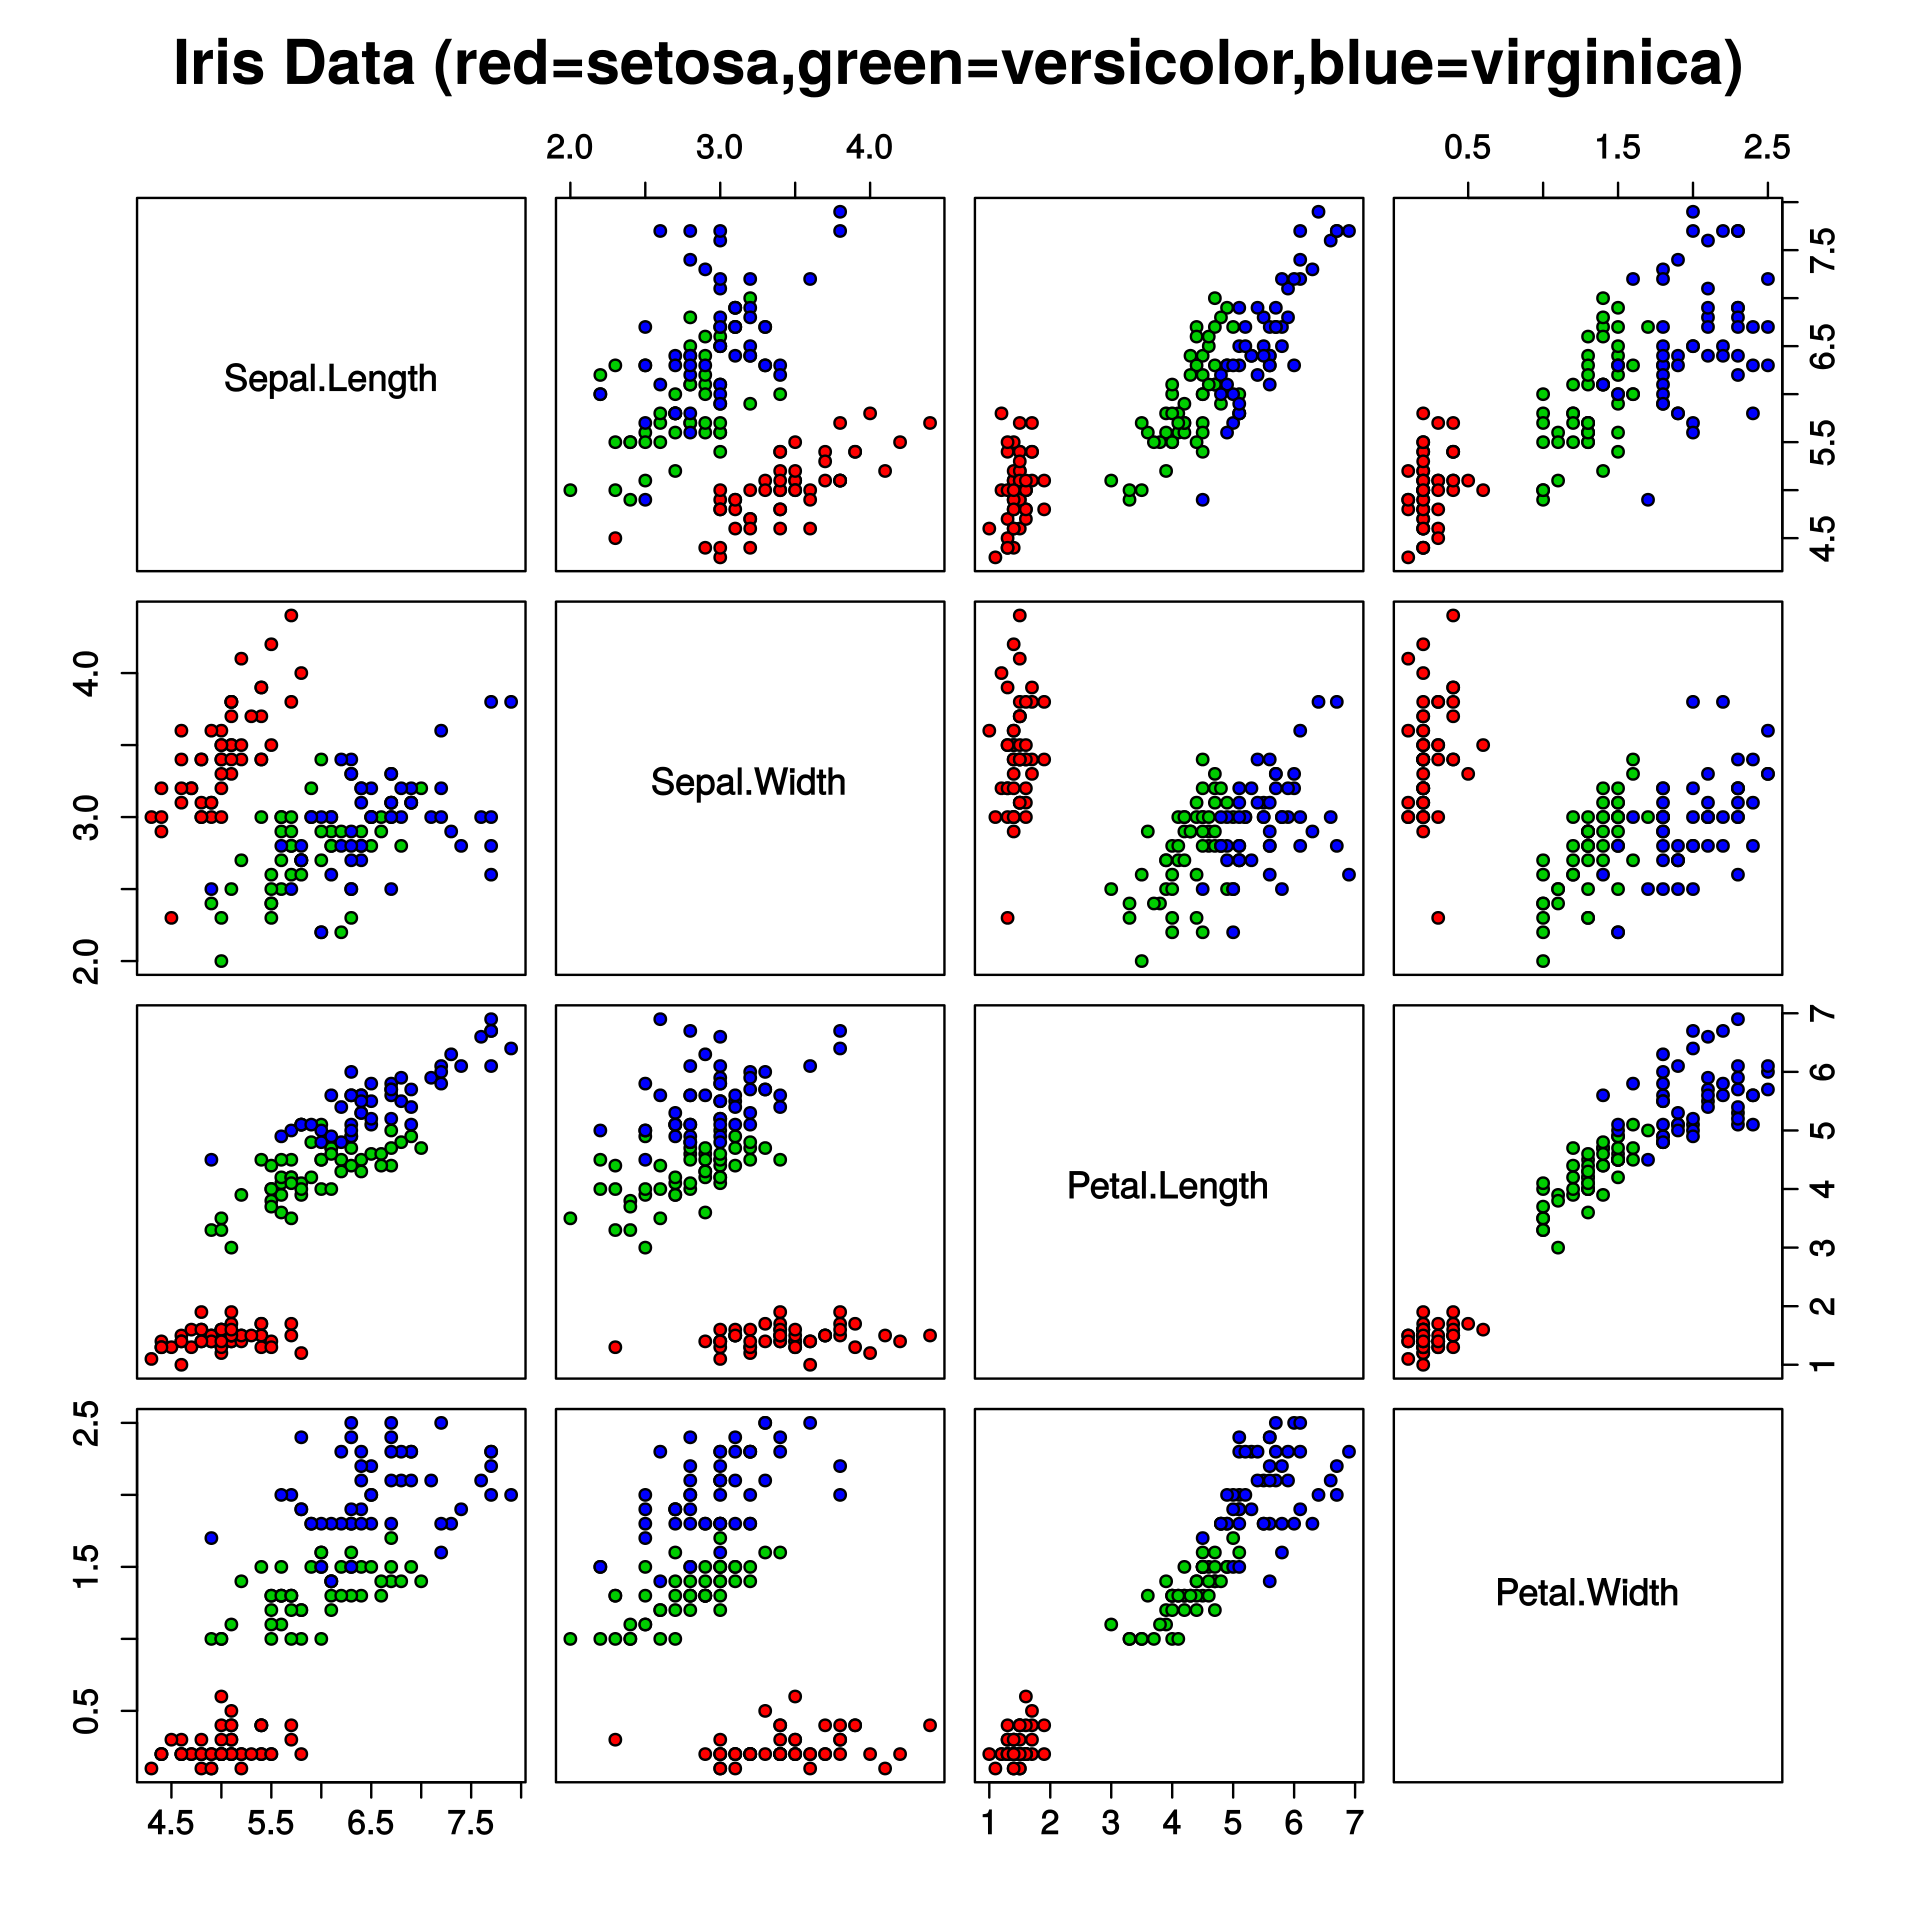
\includegraphics[width=0.9\linewidth]{figures/iris.png}
  \caption{My figure}
  \label{fig:fig01}
\end{figure}


\begin{itemize}
\item Blah
\item Blah
\end{itemize}


\section{Research Questions}
Blah

\begin{itemize}
\item Blah 
\end{itemize}

\section{Thesis Structure}
Blah

\begin{itemize}
\item Blah 
\item Blah 
\end{itemize}



\chapter{Literature Review}

\section{Introduction}
 Lorem ipsum dolor sit amet, faucibus lorem id, nec vel curabitur fusce feugiat. Cupiditate sollicitudin delectus turpis at tincidunt ut, lorem volutpat praesent massa vivamus justo, semper magna, ipsum eros gravida vestibulum dolor lorem expedita. Tellus ac pretium feugiat massa, praesent tincidunt curabitur gravida lorem sed nisl, eu hac sit eaque pede aenean, suspendisse aenean tincidunt suspendisse ut scelerisque, fringilla magna natoque ipsum ac. Eget mattis. Nunc donec magna augue, venenatis proin commodo non feugiat mauris, mollis sodales accumsan dignissim eget, suscipit nisl imperdiet nibh integer, duis nunc dolor hac. Ac sem. Nulla ut fames dolorem, donec at tortor posuere.
 
\section{Topic 1}
 Lorem ipsum dolor sit amet, faucibus lorem id, nec vel curabitur fusce feugiat. Cupiditate sollicitudin delectus turpis at tincidunt ut, lorem volutpat praesent massa vivamus justo, semper magna, ipsum eros gravida vestibulum dolor lorem expedita. Tellus ac pretium feugiat massa, praesent tincidunt curabitur gravida lorem sed nisl, eu hac sit eaque pede aenean, suspendisse aenean tincidunt suspendisse ut scelerisque, fringilla magna natoque ipsum ac. Eget mattis. Nunc donec magna augue, venenatis proin commodo non feugiat mauris, mollis sodales accumsan dignissim eget, suscipit nisl imperdiet nibh integer, duis nunc dolor hac. Ac sem. Nulla ut fames dolorem, donec at tortor posuere.
 
 \section{conclusions}
  Lorem ipsum dolor sit amet, faucibus lorem id, nec vel curabitur fusce feugiat. Cupiditate sollicitudin delectus turpis at tincidunt ut, lorem volutpat praesent massa vivamus justo, semper magna, ipsum eros gravida vestibulum dolor lorem expedita. Tellus ac pretium feugiat massa, praesent tincidunt curabitur gravida lorem sed nisl, eu hac sit eaque pede aenean, suspendisse aenean tincidunt suspendisse ut scelerisque, fringilla magna natoque ipsum ac. Eget mattis. Nunc donec magna augue, venenatis proin commodo non feugiat mauris, mollis sodales accumsan dignissim eget, suscipit nisl imperdiet nibh integer, duis nunc dolor hac. Ac sem. Nulla ut fames dolorem, donec at tortor posuere.
\chapter{Design}
\section{Introduction}
 Lorem ipsum dolor sit amet, faucibus lorem id, nec vel curabitur fusce feugiat. Cupiditate sollicitudin delectus turpis at tincidunt ut, lorem volutpat praesent massa vivamus justo, semper magna, ipsum eros gravida vestibulum dolor lorem expedita. Tellus ac pretium feugiat massa, praesent tincidunt curabitur gravida lorem sed nisl, eu hac sit eaque pede aenean, suspendisse aenean tincidunt suspendisse ut scelerisque, fringilla magna natoque ipsum ac. Eget mattis. Nunc donec magna augue, venenatis proin commodo non feugiat mauris, mollis sodales accumsan dignissim eget, suscipit nisl imperdiet nibh integer, duis nunc dolor hac. Ac sem. Nulla ut fames dolorem, donec at tortor posuere.
 
 \section{Design}
 
 Lorem ipsum dolor sit amet, faucibus lorem id, nec vel curabitur fusce feugiat. Cupiditate sollicitudin delectus turpis at tincidunt ut, lorem volutpat praesent massa vivamus justo, semper magna, ipsum eros gravida vestibulum dolor lorem expedita. Tellus ac pretium feugiat massa, praesent tincidunt curabitur gravida lorem sed nisl, eu hac sit eaque pede aenean, suspendisse aenean tincidunt suspendisse ut scelerisque, fringilla magna natoque ipsum ac. Eget mattis. Nunc donec magna augue, venenatis proin commodo non feugiat mauris, mollis sodales accumsan dignissim eget, suscipit nisl imperdiet nibh integer, duis nunc dolor hac. Ac sem. Nulla ut fames dolorem, donec at tortor posuere. In Table \ref{tab:tab01}.
 
 
 \begin{table}[]
\begin{tabular}{lll}
Security features     & Handling Security Service & References \\
\hline
Key 1         & Auth 1            & 5, 5  \\  
Key 2         & Auth 2            & 7, 5  \\ 
Key 3         & Auth 3             & 4, 5  \\ 
\end{tabular}\label{tab:tab01}\caption{My table}
\end{table}
  
  \subsection{Sub-design}
Lorem ipsum dolor sit amet, faucibus lorem id, nec vel curabitur fusce feugiat. Cupiditate sollicitudin delectus turpis at tincidunt ut, lorem volutpat praesent massa vivamus justo, semper magna, ipsum eros gravida vestibulum dolor lorem expedita. Tellus ac pretium feugiat massa, praesent tincidunt curabitur gravida lorem sed nisl, eu hac sit eaque pede aenean, suspendisse aenean tincidunt suspendisse ut scelerisque, fringilla magna natoque ipsum ac. Eget mattis. Nunc donec magna augue, venenatis proin commodo non feugiat mauris, mollis sodales accumsan dignissim eget, suscipit nisl imperdiet nibh integer, duis nunc dolor hac. Ac sem. Nulla ut fames dolorem, donec at tortor posuere.
 
  
  \section{Conclusions}
 Lorem ipsum dolor sit amet, faucibus lorem id, nec vel curabitur fusce feugiat. Cupiditate sollicitudin delectus turpis at tincidunt ut, lorem volutpat praesent massa vivamus justo, semper magna, ipsum eros gravida vestibulum dolor lorem expedita. Tellus ac pretium feugiat massa, praesent tincidunt curabitur gravida lorem sed nisl, eu hac sit eaque pede aenean, suspendisse aenean tincidunt suspendisse ut scelerisque, fringilla magna natoque ipsum ac. Eget mattis. Nunc donec magna augue, venenatis proin commodo non feugiat mauris, mollis sodales accumsan dignissim eget, suscipit nisl imperdiet nibh integer, duis nunc dolor hac. Ac sem. Nulla ut fames dolorem, donec at tortor posuere.

\chapter{Implementation}

\section{Intoduction}
 Lorem ipsum dolor sit amet, faucibus lorem id, nec vel curabitur fusce feugiat. Cupiditate sollicitudin delectus turpis at tincidunt ut, lorem volutpat praesent massa vivamus justo, semper magna, ipsum eros gravida vestibulum dolor lorem expedita. Tellus ac pretium feugiat massa, praesent tincidunt curabitur gravida lorem sed nisl, eu hac sit eaque pede aenean, suspendisse aenean tincidunt suspendisse ut scelerisque, fringilla magna natoque ipsum ac. Eget mattis. Nunc donec magna augue, venenatis proin commodo non feugiat mauris, mollis sodales accumsan dignissim eget, suscipit nisl imperdiet nibh integer, duis nunc dolor hac. Ac sem. Nulla ut fames dolorem, donec at tortor posuere.
  
  
  \section{Conclusions}
Lorem ipsum dolor sit amet, faucibus lorem id, nec vel curabitur fusce feugiat. Cupiditate sollicitudin delectus turpis at tincidunt ut, lorem volutpat praesent massa vivamus justo, semper magna, ipsum eros gravida vestibulum dolor lorem expedita. Tellus ac pretium feugiat massa, praesent tincidunt curabitur gravida lorem sed nisl, eu hac sit eaque pede aenean, suspendisse aenean tincidunt suspendisse ut scelerisque, fringilla magna natoque ipsum ac. Eget mattis. Nunc donec magna augue, venenatis proin commodo non feugiat mauris, mollis sodales accumsan dignissim eget, suscipit nisl imperdiet nibh integer, duis nunc dolor hac. Ac sem. Nulla ut fames dolorem, donec at tortor posuere.

\chapter{Evaluation}
\section{Introduction}
 Lorem ipsum dolor sit amet, faucibus lorem id, nec vel curabitur fusce feugiat. Cupiditate sollicitudin delectus turpis at tincidunt ut, lorem volutpat praesent massa vivamus justo, semper magna, ipsum eros gravida vestibulum dolor lorem expedita. Tellus ac pretium feugiat massa, praesent tincidunt curabitur gravida lorem sed nisl, eu hac sit eaque pede aenean, suspendisse aenean tincidunt suspendisse ut scelerisque, fringilla magna natoque ipsum ac. Eget mattis. Nunc donec magna augue, venenatis proin commodo non feugiat mauris, mollis sodales accumsan dignissim eget, suscipit nisl imperdiet nibh integer, duis nunc dolor hac. Ac sem. Nulla ut fames dolorem, donec at tortor posuere.
  
  \section{Conclusions}
Lorem ipsum dolor sit amet, faucibus lorem id, nec vel curabitur fusce feugiat. Cupiditate sollicitudin delectus turpis at tincidunt ut, lorem volutpat praesent massa vivamus justo, semper magna, ipsum eros gravida vestibulum dolor lorem expedita. Tellus ac pretium feugiat massa, praesent tincidunt curabitur gravida lorem sed nisl, eu hac sit eaque pede aenean, suspendisse aenean tincidunt suspendisse ut scelerisque, fringilla magna natoque ipsum ac. Eget mattis. Nunc donec magna augue, venenatis proin commodo non feugiat mauris, mollis sodales accumsan dignissim eget, suscipit nisl imperdiet nibh integer, duis nunc dolor hac. Ac sem. Nulla ut fames dolorem, donec at tortor posuere.

\chapter{Conclusions}
\section{Main Conclusions}
 Lorem ipsum dolor sit amet, faucibus lorem id, nec vel curabitur fusce feugiat. Cupiditate sollicitudin delectus turpis at tincidunt ut, lorem volutpat praesent massa vivamus justo, semper magna, ipsum eros gravida vestibulum dolor lorem expedita. Tellus ac pretium feugiat massa, praesent tincidunt curabitur gravida lorem sed nisl, eu hac sit eaque pede aenean, suspendisse aenean tincidunt suspendisse ut scelerisque, fringilla magna natoque ipsum ac. Eget mattis. Nunc donec magna augue, venenatis proin commodo non feugiat mauris, mollis sodales accumsan dignissim eget, suscipit nisl imperdiet nibh integer, duis nunc dolor hac. Ac sem. Nulla ut fames dolorem, donec at tortor posuere.
\section{Delivery against objectives}
 Lorem ipsum dolor sit amet, faucibus lorem id, nec vel curabitur fusce feugiat. Cupiditate sollicitudin delectus turpis at tincidunt ut, lorem volutpat praesent massa vivamus justo, semper magna, ipsum eros gravida vestibulum dolor lorem expedita. Tellus ac pretium feugiat massa, praesent tincidunt curabitur gravida lorem sed nisl, eu hac sit eaque pede aenean, suspendisse aenean tincidunt suspendisse ut scelerisque, fringilla magna natoque ipsum ac. Eget mattis. Nunc donec magna augue, venenatis proin commodo non feugiat mauris, mollis sodales accumsan dignissim eget, suscipit nisl imperdiet nibh integer, duis nunc dolor hac. Ac sem. Nulla ut fames dolorem, donec at tortor posuere.
\section{Future work}
 Lorem ipsum dolor sit amet, faucibus lorem id, nec vel curabitur fusce feugiat. Cupiditate sollicitudin delectus turpis at tincidunt ut, lorem volutpat praesent massa vivamus justo, semper magna, ipsum eros gravida vestibulum dolor lorem expedita. Tellus ac pretium feugiat massa, praesent tincidunt curabitur gravida lorem sed nisl, eu hac sit eaque pede aenean, suspendisse aenean tincidunt suspendisse ut scelerisque, fringilla magna natoque ipsum ac. Eget mattis. Nunc donec magna augue, venenatis proin commodo non feugiat mauris, mollis sodales accumsan dignissim eget, suscipit nisl imperdiet nibh integer, duis nunc dolor hac. Ac sem. Nulla ut fames dolorem, donec at tortor posuere.
\section{Personal reflection}
 Lorem ipsum dolor sit amet, faucibus lorem id, nec vel curabitur fusce feugiat. Cupiditate sollicitudin delectus turpis at tincidunt ut, lorem volutpat praesent massa vivamus justo, semper magna, ipsum eros gravida vestibulum dolor lorem expedita. Tellus ac pretium feugiat massa, praesent tincidunt curabitur gravida lorem sed nisl, eu hac sit eaque pede aenean, suspendisse aenean tincidunt suspendisse ut scelerisque, fringilla magna natoque ipsum ac. Eget mattis. Nunc donec magna augue, venenatis proin commodo non feugiat mauris, mollis sodales accumsan dignissim eget, suscipit nisl imperdiet nibh integer, duis nunc dolor hac. Ac sem. Nulla ut fames dolorem, donec at tortor posuere.


\renewcommand\bibname{References}
\bibliography{mybib}
\bibliographystyle{apalike}
\clearpage
%you will need to run the makeglossaries command if you are using a local installation of Latex to get the glossary to be printed.
\printglossary[type=\acronymtype]
\printglossary
\clearpage
%appendices come after the references and glossary
\end{document}
